\begin{center}

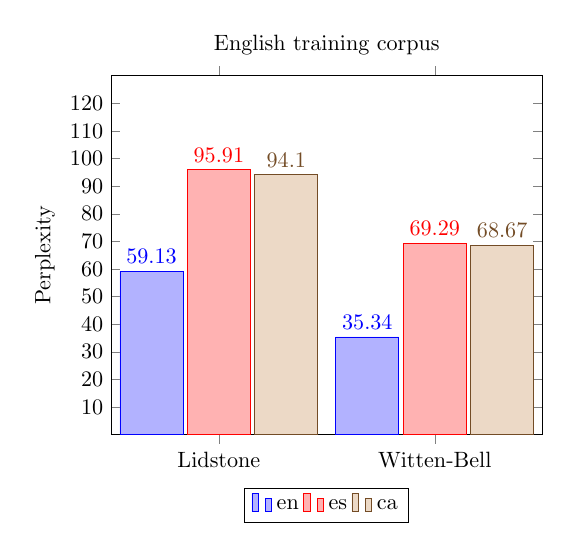
\begin{tikzpicture}[scale=.8]
\begin{axis}[
	title={English training corpus},
	ybar,
	enlarge x limits=0.5,
	legend style={at={(0.5,-0.15)}, anchor=north,legend columns=-1},
	ylabel={Perplexity},
	symbolic x coords={Lidstone,Witten-Bell},
	xtick=data,
	ymin=0, ymax=130,
	ytick={10,20,30,40,50,60,70,80,90,100,110,120},
	bar width=1cm,
	nodes near coords,
]
\addplot coordinates {(Lidstone,59.1283089317215982) (Witten-Bell,35.3392196020463203)};
\addplot coordinates {(Lidstone,95.9125002627099690) (Witten-Bell,69.2914739187706914)};
\addplot coordinates {(Lidstone,94.1046507794276152) (Witten-Bell,68.6735491041301742)};
\legend{en,es,ca}
\end{axis}
\end{tikzpicture}
\qquad
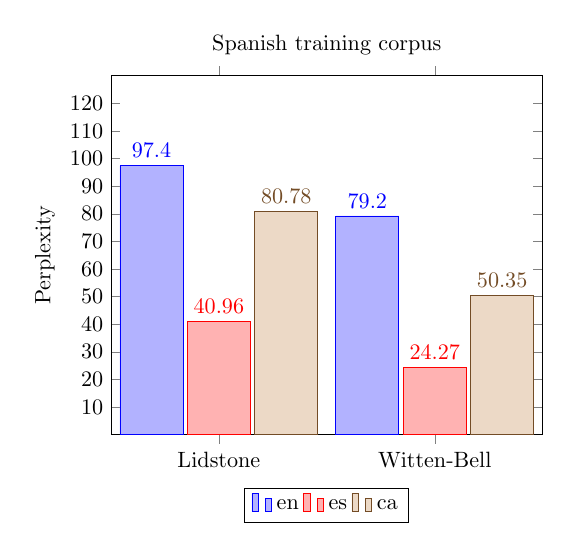
\begin{tikzpicture}[scale=.8]
\begin{axis}[
	title={Spanish training corpus},
	ybar,
	enlarge x limits=0.5,
	legend style={at={(0.5,-0.15)}, anchor=north,legend columns=-1},
	ylabel={Perplexity},
	symbolic x coords={Lidstone,Witten-Bell},
	xtick=data,
	ymin=0, ymax=130,
	ytick={10,20,30,40,50,60,70,80,90,100,110,120},
	bar width=1cm,
	nodes near coords,
]
\addplot coordinates {(Lidstone,97.4011888994087229) (Witten-Bell,79.2032399414232628)};
\addplot coordinates {(Lidstone,40.9639438998515004) (Witten-Bell,24.2690525366963570)};
\addplot coordinates {(Lidstone,80.7829345245770583) (Witten-Bell,50.3545705852040442)};
\legend{en,es,ca}
\end{axis}
\end{tikzpicture}

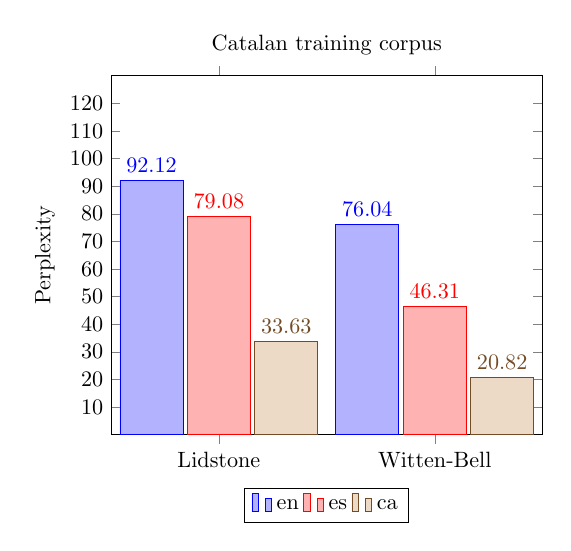
\begin{tikzpicture}[scale=.8]
\begin{axis}[
	title={Catalan training corpus},
	ybar,
	enlarge x limits=0.5,
	legend style={at={(0.5,-0.15)}, anchor=north,legend columns=-1},
	ylabel={Perplexity},
	symbolic x coords={Lidstone,Witten-Bell},
	xtick=data,
	ymin=0, ymax=130,
	ytick={10,20,30,40,50,60,70,80,90,100,110,120},
	bar width=1cm,
	nodes near coords,
]
\addplot coordinates {(Lidstone,92.1240701265360258) (Witten-Bell,76.0432071881298270)};
\addplot coordinates {(Lidstone,79.0766895724054990) (Witten-Bell,46.3116987920521836)};
\addplot coordinates {(Lidstone,33.6300430098770633) (Witten-Bell,20.8166778217064490)};
\legend{en,es,ca}
\end{axis}
\end{tikzpicture}

\end{center}